\documentclass[1p]{elsarticle_modified}
%\bibliographystyle{elsarticle-num}

%\usepackage[colorlinks]{hyperref}
%\usepackage{abbrmath_seonhwa} %\Abb, \Ascr, \Acal ,\Abf, \Afrak
\usepackage{amsfonts}
\usepackage{amssymb}
\usepackage{amsmath}
\usepackage{amsthm}
\usepackage{scalefnt}
\usepackage{amsbsy}
\usepackage{kotex}
\usepackage{caption}
\usepackage{subfig}
\usepackage{color}
\usepackage{graphicx}
\usepackage{xcolor} %% white, black, red, green, blue, cyan, magenta, yellow
\usepackage{float}
\usepackage{setspace}
\usepackage{hyperref}

\usepackage{tikz}
\usetikzlibrary{arrows}

\usepackage{multirow}
\usepackage{array} % fixed length table
\usepackage{hhline}

%%%%%%%%%%%%%%%%%%%%%
\makeatletter
\renewcommand*\env@matrix[1][\arraystretch]{%
	\edef\arraystretch{#1}%
	\hskip -\arraycolsep
	\let\@ifnextchar\new@ifnextchar
	\array{*\c@MaxMatrixCols c}}
\makeatother %https://tex.stackexchange.com/questions/14071/how-can-i-increase-the-line-spacing-in-a-matrix
%%%%%%%%%%%%%%%

\usepackage[normalem]{ulem}

\newcommand{\msout}[1]{\ifmmode\text{\sout{\ensuremath{#1}}}\else\sout{#1}\fi}
%SOURCE: \msout is \stkout macro in https://tex.stackexchange.com/questions/20609/strikeout-in-math-mode

\newcommand{\cancel}[1]{
	\ifmmode
	{\color{red}\msout{#1}}
	\else
	{\color{red}\sout{#1}}
	\fi
}

\newcommand{\add}[1]{
	{\color{blue}\uwave{#1}}
}

\newcommand{\replace}[2]{
	\ifmmode
	{\color{red}\msout{#1}}{\color{blue}\uwave{#2}}
	\else
	{\color{red}\sout{#1}}{\color{blue}\uwave{#2}}
	\fi
}

\newcommand{\Sol}{\mathcal{S}} %segment
\newcommand{\D}{D} %diagram
\newcommand{\A}{\mathcal{A}} %arc


%%%%%%%%%%%%%%%%%%%%%%%%%%%%%5 test

\def\sl{\operatorname{\textup{SL}}(2,\Cbb)}
\def\psl{\operatorname{\textup{PSL}}(2,\Cbb)}
\def\quan{\mkern 1mu \triangleright \mkern 1mu}

\theoremstyle{definition}
\newtheorem{thm}{Theorem}[section]
\newtheorem{prop}[thm]{Proposition}
\newtheorem{lem}[thm]{Lemma}
\newtheorem{ques}[thm]{Question}
\newtheorem{cor}[thm]{Corollary}
\newtheorem{defn}[thm]{Definition}
\newtheorem{exam}[thm]{Example}
\newtheorem{rmk}[thm]{Remark}
\newtheorem{alg}[thm]{Algorithm}

\newcommand{\I}{\sqrt{-1}}
\begin{document}

%\begin{frontmatter}
%
%\title{Boundary parabolic representations of knots up to 8 crossings}
%
%%% Group authors per affiliation:
%\author{Yunhi Cho} 
%\address{Department of Mathematics, University of Seoul, Seoul, Korea}
%\ead{yhcho@uos.ac.kr}
%
%
%\author{Seonhwa Kim} %\fnref{s_kim}}
%\address{Center for Geometry and Physics, Institute for Basic Science, Pohang, 37673, Korea}
%\ead{ryeona17@ibs.re.kr}
%
%\author{Hyuk Kim}
%\address{Department of Mathematical Sciences, Seoul National University, Seoul 08826, Korea}
%\ead{hyukkim@snu.ac.kr}
%
%\author{Seokbeom Yoon}
%\address{Department of Mathematical Sciences, Seoul National University, Seoul, 08826,  Korea}
%\ead{sbyoon15@snu.ac.kr}
%
%\begin{abstract}
%We find all boundary parabolic representation of knots up to 8 crossings.
%
%\end{abstract}
%\begin{keyword}
%    \MSC[2010] 57M25 
%\end{keyword}
%
%\end{frontmatter}

%\linenumbers
%\tableofcontents
%
\newcommand\colored[1]{\textcolor{white}{\rule[-0.35ex]{0.8em}{1.4ex}}\kern-0.8em\color{red} #1}%
%\newcommand\colored[1]{\textcolor{white}{ #1}\kern-2.17ex	\textcolor{white}{ #1}\kern-1.81ex	\textcolor{white}{ #1}\kern-2.15ex\color{red}#1	}

{\Large $\underline{12n_{0669}~(K12n_{0669})}$}

\setlength{\tabcolsep}{10pt}
\renewcommand{\arraystretch}{1.6}
\vspace{1cm}\begin{tabular}{m{100pt}>{\centering\arraybackslash}m{274pt}}
\multirow{5}{120pt}{
	\centering
	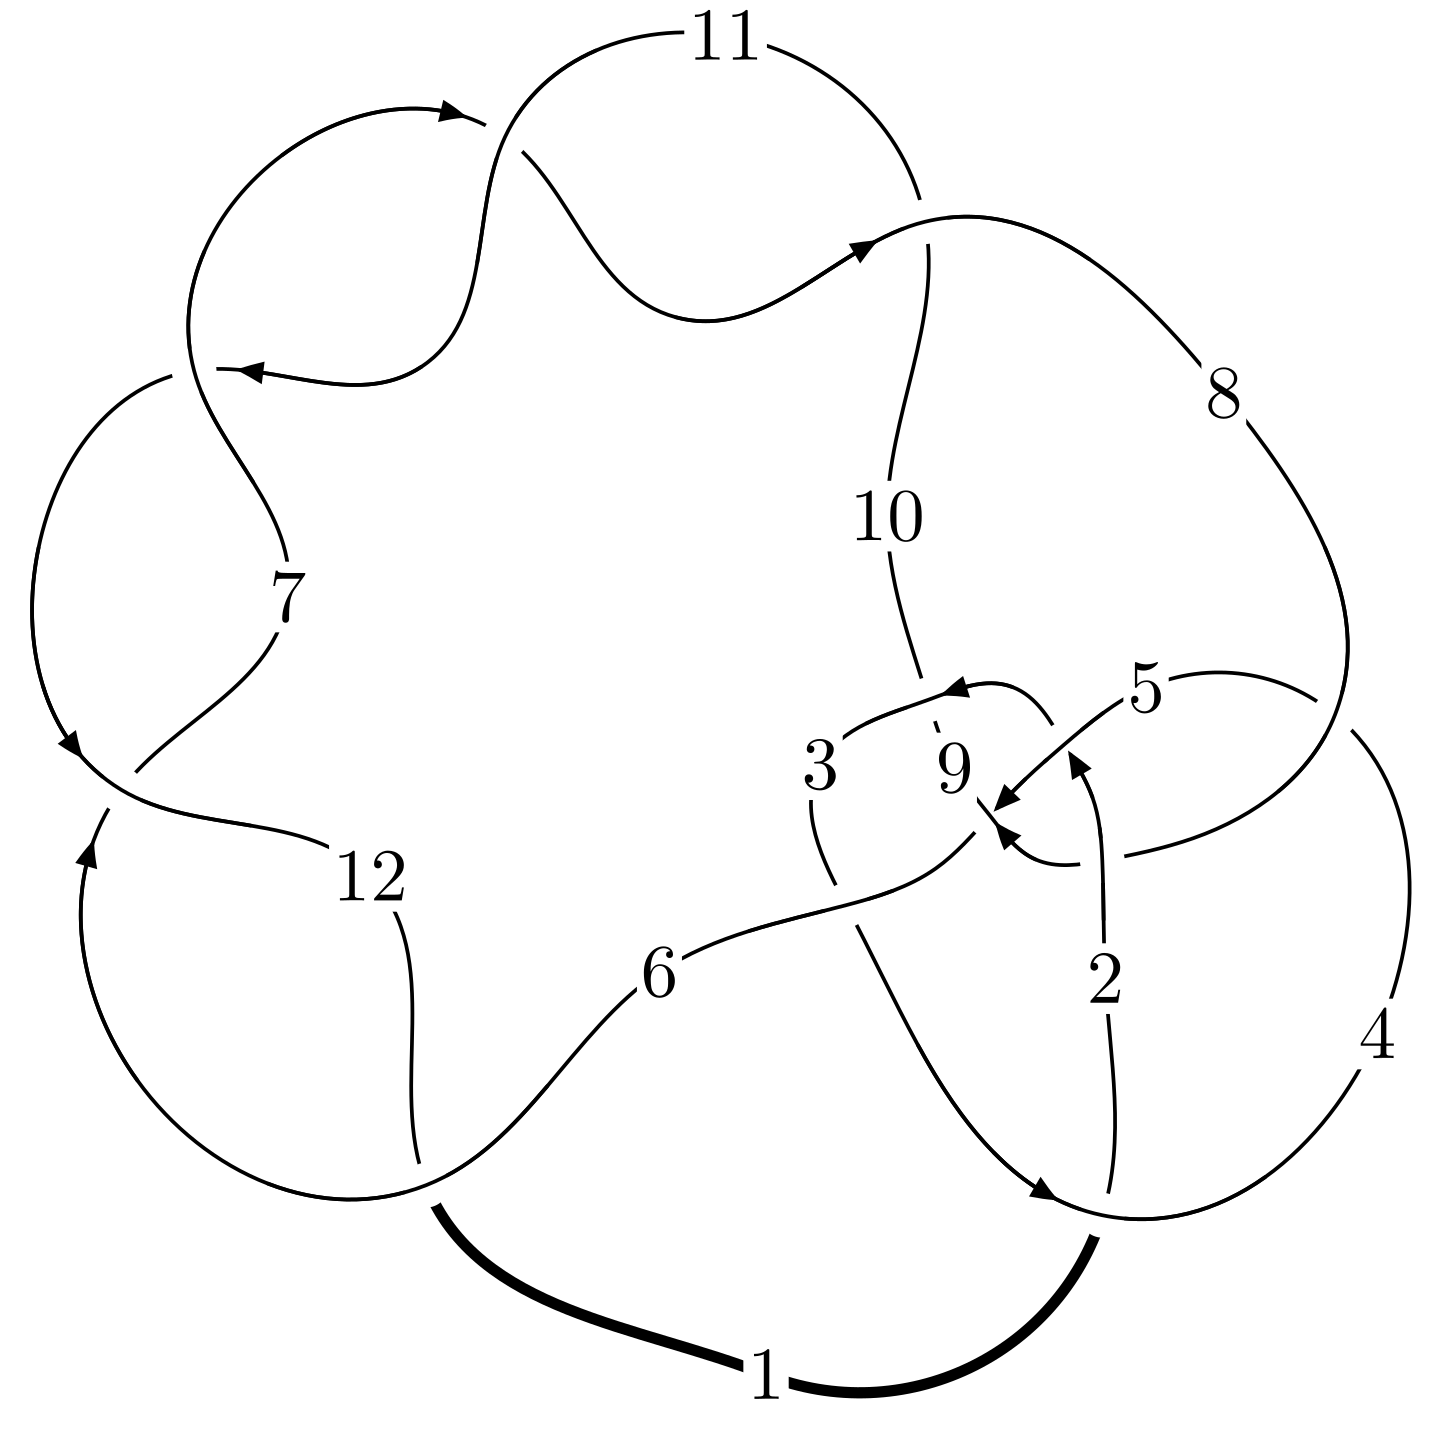
\includegraphics[width=112pt]{../../../GIT/diagram.site/Diagrams/png/2758_12n_0669.png}\\
\ \ \ A knot diagram\footnotemark}&
\allowdisplaybreaks
\textbf{Linearized knot diagam} \\
\cline{2-2}
 &
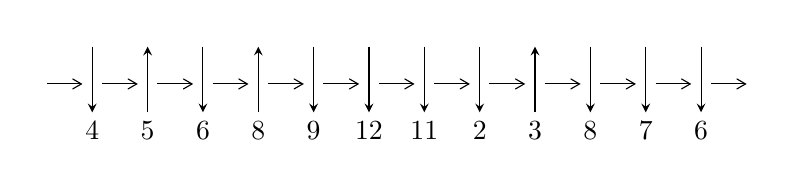
\begin{tikzpicture}[x=20pt, y=17pt]
	% nodes
	\node (C0) at (0, 0) {};
	\node (C1) at (1, 0) {};
	\node (C1U) at (1, +1) {};
	\node (C1D) at (1, -1) {4};

	\node (C2) at (2, 0) {};
	\node (C2U) at (2, +1) {};
	\node (C2D) at (2, -1) {5};

	\node (C3) at (3, 0) {};
	\node (C3U) at (3, +1) {};
	\node (C3D) at (3, -1) {6};

	\node (C4) at (4, 0) {};
	\node (C4U) at (4, +1) {};
	\node (C4D) at (4, -1) {8};

	\node (C5) at (5, 0) {};
	\node (C5U) at (5, +1) {};
	\node (C5D) at (5, -1) {9};

	\node (C6) at (6, 0) {};
	\node (C6U) at (6, +1) {};
	\node (C6D) at (6, -1) {12};

	\node (C7) at (7, 0) {};
	\node (C7U) at (7, +1) {};
	\node (C7D) at (7, -1) {11};

	\node (C8) at (8, 0) {};
	\node (C8U) at (8, +1) {};
	\node (C8D) at (8, -1) {2};

	\node (C9) at (9, 0) {};
	\node (C9U) at (9, +1) {};
	\node (C9D) at (9, -1) {3};

	\node (C10) at (10, 0) {};
	\node (C10U) at (10, +1) {};
	\node (C10D) at (10, -1) {8};

	\node (C11) at (11, 0) {};
	\node (C11U) at (11, +1) {};
	\node (C11D) at (11, -1) {7};

	\node (C12) at (12, 0) {};
	\node (C12U) at (12, +1) {};
	\node (C12D) at (12, -1) {6};
	\node (C13) at (13, 0) {};

	% arrows
	\draw[->,>={angle 60}]
	(C0) edge (C1) (C1) edge (C2) (C2) edge (C3) (C3) edge (C4) (C4) edge (C5) (C5) edge (C6) (C6) edge (C7) (C7) edge (C8) (C8) edge (C9) (C9) edge (C10) (C10) edge (C11) (C11) edge (C12) (C12) edge (C13) ;	\draw[->,>=stealth]
	(C1U) edge (C1D) (C2D) edge (C2U) (C3U) edge (C3D) (C4D) edge (C4U) (C5U) edge (C5D) (C6U) edge (C6D) (C7U) edge (C7D) (C8U) edge (C8D) (C9D) edge (C9U) (C10U) edge (C10D) (C11U) edge (C11D) (C12U) edge (C12D) ;
	\end{tikzpicture} \\
\hhline{~~} \\& 
\textbf{Solving Sequence} \\ \cline{2-2} 
 &
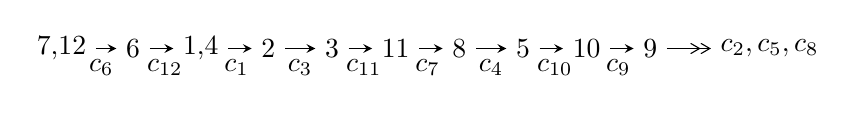
\begin{tikzpicture}[x=23pt, y=7pt]
	% node
	\node (A0) at (-1/8, 0) {7,12};
	\node (A1) at (1, 0) {6};
	\node (A2) at (33/16, 0) {1,4};
	\node (A3) at (25/8, 0) {2};
	\node (A4) at (33/8, 0) {3};
	\node (A5) at (41/8, 0) {11};
	\node (A6) at (49/8, 0) {8};
	\node (A7) at (57/8, 0) {5};
	\node (A8) at (65/8, 0) {10};
	\node (A9) at (73/8, 0) {9};
	\node (C1) at (1/2, -1) {$c_{6}$};
	\node (C2) at (3/2, -1) {$c_{12}$};
	\node (C3) at (21/8, -1) {$c_{1}$};
	\node (C4) at (29/8, -1) {$c_{3}$};
	\node (C5) at (37/8, -1) {$c_{11}$};
	\node (C6) at (45/8, -1) {$c_{7}$};
	\node (C7) at (53/8, -1) {$c_{4}$};
	\node (C8) at (61/8, -1) {$c_{10}$};
	\node (C9) at (69/8, -1) {$c_{9}$};
	\node (A10) at (11, 0) {$c_{2},c_{5},c_{8}$};

	% edge
	\draw[->,>=stealth]	
	(A0) edge (A1) (A1) edge (A2) (A2) edge (A3) (A3) edge (A4) (A4) edge (A5) (A5) edge (A6) (A6) edge (A7) (A7) edge (A8) (A8) edge (A9) ;
	\draw[->>,>={angle 60}]	
	(A9) edge (A10);
\end{tikzpicture} \\ 

\end{tabular} \\

\footnotetext{
The image of knot diagram is generated by the software ``\textbf{Draw programme}" developed by Andrew Bartholomew(\url{http://www.layer8.co.uk/maths/draw/index.htm\#Running-draw}), where we modified some parts for our purpose(\url{https://github.com/CATsTAILs/LinksPainter}).
}\phantom \\ \newline 
\centering \textbf{Ideals for irreducible components\footnotemark of $X_{\text{par}}$} 
 
\begin{align*}
I^u_{1}&=\langle 
-99 u^{27}-595 u^{26}+\cdots+181 b-1270,\;-7972 u^{27}-42371 u^{26}+\cdots+11403 a-75384,\\
\phantom{I^u_{1}}&\phantom{= \langle  }u^{28}+5 u^{27}+\cdots+18 u+9\rangle \\
I^u_{2}&=\langle 
- u^{15} a-13 u^{15}+\cdots+a-9,\;u^{14} a+u^{15}+\cdots+a+2,\;u^{16}-3 u^{15}+\cdots+4 u^2+1\rangle \\
I^u_{3}&=\langle 
- u^{11}+3 u^{10}-11 u^9+22 u^8-41 u^7+55 u^6-63 u^5+54 u^4-37 u^3+18 u^2+b-6 u+1,\\
\phantom{I^u_{3}}&\phantom{= \langle  }- u^{11}+2 u^{10}-9 u^9+13 u^8-27 u^7+26 u^6-29 u^5+13 u^4-4 u^3-7 u^2+a+4 u-4,\\
\phantom{I^u_{3}}&\phantom{= \langle  }u^{12}-2 u^{11}+10 u^{10}-16 u^9+37 u^8-46 u^7+62 u^6-56 u^5+46 u^4-25 u^3+13 u^2-2 u+1\rangle \\
\\
I^v_{1}&=\langle 
a,\;b-1,\;v-1\rangle \\
\end{align*}
\raggedright * 4 irreducible components of $\dim_{\mathbb{C}}=0$, with total 73 representations.\\
\footnotetext{All coefficients of polynomials are rational numbers. But the coefficients are sometimes approximated in decimal forms when there is not enough margin.}
\newpage
\renewcommand{\arraystretch}{1}
\centering \section*{I. $I^u_{1}= \langle -99 u^{27}-595 u^{26}+\cdots+181 b-1270,\;-7972 u^{27}-42371 u^{26}+\cdots+11403 a-75384,\;u^{28}+5 u^{27}+\cdots+18 u+9 \rangle$}
\flushleft \textbf{(i) Arc colorings}\\
\begin{tabular}{m{7pt} m{180pt} m{7pt} m{180pt} }
\flushright $a_{7}=$&$\begin{pmatrix}1\\0\end{pmatrix}$ \\
\flushright $a_{12}=$&$\begin{pmatrix}0\\u\end{pmatrix}$ \\
\flushright $a_{6}=$&$\begin{pmatrix}1\\- u^2\end{pmatrix}$ \\
\flushright $a_{1}=$&$\begin{pmatrix}- u\\u^3+u\end{pmatrix}$ \\
\flushright $a_{4}=$&$\begin{pmatrix}0.699114 u^{27}+3.71578 u^{26}+\cdots+13.4910 u+6.61089\\0.546961 u^{27}+3.28729 u^{26}+\cdots+8.67956 u+7.01657\end{pmatrix}$ \\
\flushright $a_{2}=$&$\begin{pmatrix}1.45523 u^{27}+7.64395 u^{26}+\cdots+37.2140 u+25.2139\\-1.21547 u^{27}-3.08287 u^{26}+\cdots+5.82320 u+13.6298\end{pmatrix}$ \\
\flushright $a_{3}=$&$\begin{pmatrix}0.559414 u^{27}+2.93677 u^{26}+\cdots+11.9148 u+11.6456\\-0.220205 u^{27}-0.414365 u^{26}+\cdots+5.97316 u+6.29203\end{pmatrix}$ \\
\flushright $a_{11}=$&$\begin{pmatrix}u\\u\end{pmatrix}$ \\
\flushright $a_{8}=$&$\begin{pmatrix}u^2+1\\u^2\end{pmatrix}$ \\
\flushright $a_{5}=$&$\begin{pmatrix}0.419714 u^{27}+2.15777 u^{26}+\cdots+8.33868 u+6.68035\\0.122336 u^{27}+0.563536 u^{26}+\cdots-0.540647 u+3.05998\end{pmatrix}$ \\
\flushright $a_{10}=$&$\begin{pmatrix}u^3+2 u\\u^3+u\end{pmatrix}$ \\
\flushright $a_{9}=$&$\begin{pmatrix}-1.11225 u^{27}-4.07980 u^{26}+\cdots-12.1491 u-1.59984\\-0.775848 u^{27}-2.30939 u^{26}+\cdots-0.764799 u+3.32281\end{pmatrix}$\\&\end{tabular}
\flushleft \textbf{(ii) Obstruction class $= -1$}\\~\\
\flushleft \textbf{(iii) Cusp Shapes $= -\frac{1388}{1267} u^{27}-\frac{1029}{181} u^{26}+\cdots-\frac{71766}{1267} u+\frac{12063}{1267}$}\\~\\
\newpage\renewcommand{\arraystretch}{1}
\flushleft \textbf{(iv) u-Polynomials at the component}\newline \\
\begin{tabular}{m{50pt}|m{274pt}}
Crossings & \hspace{64pt}u-Polynomials at each crossing \\
\hline $$\begin{aligned}c_{1},c_{3}\end{aligned}$$&$\begin{aligned}
&u^{28}+2 u^{27}+\cdots-4 u+1
\end{aligned}$\\
\hline $$\begin{aligned}c_{2}\end{aligned}$$&$\begin{aligned}
&u^{28}+18 u^{27}+\cdots+72 u+9
\end{aligned}$\\
\hline $$\begin{aligned}c_{4},c_{9}\end{aligned}$$&$\begin{aligned}
&u^{28}-2 u^{27}+\cdots- u+8
\end{aligned}$\\
\hline $$\begin{aligned}c_{5},c_{8}\end{aligned}$$&$\begin{aligned}
&u^{28}- u^{27}+\cdots+u+1
\end{aligned}$\\
\hline $$\begin{aligned}c_{6},c_{7},c_{10}\\c_{11},c_{12}\end{aligned}$$&$\begin{aligned}
&u^{28}-5 u^{27}+\cdots-18 u+9
\end{aligned}$\\
\hline
\end{tabular}\\~\\
\newpage\renewcommand{\arraystretch}{1}
\flushleft \textbf{(v) Riley Polynomials at the component}\newline \\
\begin{tabular}{m{50pt}|m{274pt}}
Crossings & \hspace{64pt}Riley Polynomials at each crossing \\
\hline $$\begin{aligned}c_{1},c_{3}\end{aligned}$$&$\begin{aligned}
&y^{28}-34 y^{27}+\cdots-12 y+1
\end{aligned}$\\
\hline $$\begin{aligned}c_{2}\end{aligned}$$&$\begin{aligned}
&y^{28}+46 y^{26}+\cdots+1260 y+81
\end{aligned}$\\
\hline $$\begin{aligned}c_{4},c_{9}\end{aligned}$$&$\begin{aligned}
&y^{28}+10 y^{27}+\cdots+879 y+64
\end{aligned}$\\
\hline $$\begin{aligned}c_{5},c_{8}\end{aligned}$$&$\begin{aligned}
&y^{28}-11 y^{27}+\cdots-27 y+1
\end{aligned}$\\
\hline $$\begin{aligned}c_{6},c_{7},c_{10}\\c_{11},c_{12}\end{aligned}$$&$\begin{aligned}
&y^{28}+33 y^{27}+\cdots-90 y+81
\end{aligned}$\\
\hline
\end{tabular}\\~\\
\newpage\flushleft \textbf{(vi) Complex Volumes and Cusp Shapes}
$$\begin{array}{c|c|c}  
\text{Solutions to }I^u_{1}& \I (\text{vol} + \sqrt{-1}CS) & \text{Cusp shape}\\
 \hline 
\begin{aligned}
u &= \phantom{-}0.279310 + 1.005780 I \\
a &= \phantom{-}0.111453 - 0.538123 I \\
b &= -0.460280 - 0.329159 I\end{aligned}
 & \phantom{-}2.15334 - 3.08002 I & -5.41932 + 2.17495 I \\ \hline\begin{aligned}
u &= \phantom{-}0.279310 - 1.005780 I \\
a &= \phantom{-}0.111453 + 0.538123 I \\
b &= -0.460280 + 0.329159 I\end{aligned}
 & \phantom{-}2.15334 + 3.08002 I & -5.41932 - 2.17495 I \\ \hline\begin{aligned}
u &= -0.720208 + 0.617732 I \\
a &= -0.067974 - 1.221620 I \\
b &= -0.518022 + 0.676690 I\end{aligned}
 & -5.18301 + 11.95320 I & -6.36826 - 8.35721 I \\ \hline\begin{aligned}
u &= -0.720208 - 0.617732 I \\
a &= -0.067974 + 1.221620 I \\
b &= -0.518022 - 0.676690 I\end{aligned}
 & -5.18301 - 11.95320 I & -6.36826 + 8.35721 I \\ \hline\begin{aligned}
u &= -0.778368 + 0.420776 I \\
a &= \phantom{-}0.148251 - 0.811625 I \\
b &= -1.044860 + 0.185626 I\end{aligned}
 & -5.77287 - 6.98018 I & -7.82028 + 3.54637 I \\ \hline\begin{aligned}
u &= -0.778368 - 0.420776 I \\
a &= \phantom{-}0.148251 + 0.811625 I \\
b &= -1.044860 - 0.185626 I\end{aligned}
 & -5.77287 + 6.98018 I & -7.82028 - 3.54637 I \\ \hline\begin{aligned}
u &= -0.588348 + 0.532762 I \\
a &= -0.326563 + 1.326180 I \\
b &= \phantom{-}0.777651 - 0.025379 I\end{aligned}
 & -4.60494 + 0.48065 I & -11.27827 + 0.66157 I \\ \hline\begin{aligned}
u &= -0.588348 - 0.532762 I \\
a &= -0.326563 - 1.326180 I \\
b &= \phantom{-}0.777651 + 0.025379 I\end{aligned}
 & -4.60494 - 0.48065 I & -11.27827 - 0.66157 I \\ \hline\begin{aligned}
u &= -0.609349 + 0.472094 I \\
a &= \phantom{-}0.554010 + 1.282630 I \\
b &= \phantom{-}0.814858 - 0.516381 I\end{aligned}
 & -4.78529 + 3.61019 I & -12.2949 - 8.1596 I \\ \hline\begin{aligned}
u &= -0.609349 - 0.472094 I \\
a &= \phantom{-}0.554010 - 1.282630 I \\
b &= \phantom{-}0.814858 + 0.516381 I\end{aligned}
 & -4.78529 - 3.61019 I & -12.2949 + 8.1596 I\\
 \hline 
 \end{array}$$\newpage$$\begin{array}{c|c|c}  
\text{Solutions to }I^u_{1}& \I (\text{vol} + \sqrt{-1}CS) & \text{Cusp shape}\\
 \hline 
\begin{aligned}
u &= \phantom{-}0.230601 + 0.555602 I \\
a &= -0.857392 - 0.551333 I \\
b &= -0.249740 + 0.519303 I\end{aligned}
 & \phantom{-}0.39899 - 1.65572 I & -2.33445 + 5.92900 I \\ \hline\begin{aligned}
u &= \phantom{-}0.230601 - 0.555602 I \\
a &= -0.857392 + 0.551333 I \\
b &= -0.249740 - 0.519303 I\end{aligned}
 & \phantom{-}0.39899 + 1.65572 I & -2.33445 - 5.92900 I \\ \hline\begin{aligned}
u &= \phantom{-}0.02508 + 1.41638 I \\
a &= -0.74984 + 1.49379 I \\
b &= -0.20717 + 2.40362 I\end{aligned}
 & \phantom{-}3.21161 - 0.20656 I & -6.00000 - 0.51080 I \\ \hline\begin{aligned}
u &= \phantom{-}0.02508 - 1.41638 I \\
a &= -0.74984 - 1.49379 I \\
b &= -0.20717 - 2.40362 I\end{aligned}
 & \phantom{-}3.21161 + 0.20656 I & -6.00000 + 0.51080 I \\ \hline\begin{aligned}
u &= -0.29358 + 1.42827 I \\
a &= \phantom{-}1.004870 - 0.924707 I \\
b &= \phantom{-}1.49328 - 0.86181 I\end{aligned}
 & \phantom{-}0.13364 - 3.10062 I & -6.00000 + 3.00953 I \\ \hline\begin{aligned}
u &= -0.29358 - 1.42827 I \\
a &= \phantom{-}1.004870 + 0.924707 I \\
b &= \phantom{-}1.49328 + 0.86181 I\end{aligned}
 & \phantom{-}0.13364 + 3.10062 I & -6.00000 - 3.00953 I \\ \hline\begin{aligned}
u &= -0.18111 + 1.50663 I \\
a &= -0.84422 + 2.04492 I \\
b &= -1.34773 + 3.07117 I\end{aligned}
 & \phantom{-}1.71233 + 6.43075 I & -9.24234 - 8.11110 I \\ \hline\begin{aligned}
u &= -0.18111 - 1.50663 I \\
a &= -0.84422 - 2.04492 I \\
b &= -1.34773 - 3.07117 I\end{aligned}
 & \phantom{-}1.71233 - 6.43075 I & -9.24234 + 8.11110 I \\ \hline\begin{aligned}
u &= \phantom{-}0.05585 + 1.53567 I \\
a &= -0.229321 - 1.036530 I \\
b &= -1.01658 - 1.57906 I\end{aligned}
 & \phantom{-}7.40879 - 2.63530 I & \phantom{-0.000000 -}0. + 1.41712 I \\ \hline\begin{aligned}
u &= \phantom{-}0.05585 - 1.53567 I \\
a &= -0.229321 + 1.036530 I \\
b &= -1.01658 + 1.57906 I\end{aligned}
 & \phantom{-}7.40879 + 2.63530 I & \phantom{-0.000000 } 0. - 1.41712 I\\
 \hline 
 \end{array}$$\newpage$$\begin{array}{c|c|c}  
\text{Solutions to }I^u_{1}& \I (\text{vol} + \sqrt{-1}CS) & \text{Cusp shape}\\
 \hline 
\begin{aligned}
u &= \phantom{-}0.449761 + 0.053633 I \\
a &= -0.698805 - 0.615735 I \\
b &= \phantom{-}0.311401 + 0.365904 I\end{aligned}
 & -1.113100 - 0.415234 I & -10.08873 + 1.99111 I \\ \hline\begin{aligned}
u &= \phantom{-}0.449761 - 0.053633 I \\
a &= -0.698805 + 0.615735 I \\
b &= \phantom{-}0.311401 - 0.365904 I\end{aligned}
 & -1.113100 + 0.415234 I & -10.08873 - 1.99111 I \\ \hline\begin{aligned}
u &= -0.17350 + 1.54958 I \\
a &= -1.34694 + 1.07933 I \\
b &= -2.24580 + 1.72156 I\end{aligned}
 & \phantom{-}2.33140 + 3.21187 I & -6.00000 + 0. I\phantom{ +0.000000I} \\ \hline\begin{aligned}
u &= -0.17350 - 1.54958 I \\
a &= -1.34694 - 1.07933 I \\
b &= -2.24580 - 1.72156 I\end{aligned}
 & \phantom{-}2.33140 - 3.21187 I & -6.00000 + 0. I\phantom{ +0.000000I} \\ \hline\begin{aligned}
u &= -0.24174 + 1.57099 I \\
a &= \phantom{-}0.93340 - 1.79161 I \\
b &= \phantom{-}1.98417 - 2.74478 I\end{aligned}
 & \phantom{-}2.0404 + 15.5256 I & -6.00000 - 8.00298 I \\ \hline\begin{aligned}
u &= -0.24174 - 1.57099 I \\
a &= \phantom{-}0.93340 + 1.79161 I \\
b &= \phantom{-}1.98417 + 2.74478 I\end{aligned}
 & \phantom{-}2.0404 - 15.5256 I & -6.00000 + 8.00298 I \\ \hline\begin{aligned}
u &= \phantom{-}0.04560 + 1.71954 I \\
a &= \phantom{-}0.369072 - 0.185559 I \\
b &= \phantom{-}0.708836 - 0.625204 I\end{aligned}
 & \phantom{-}11.93830 - 4.23690 I & \phantom{-0.000000 } 0 \\ \hline\begin{aligned}
u &= \phantom{-}0.04560 - 1.71954 I \\
a &= \phantom{-}0.369072 + 0.185559 I \\
b &= \phantom{-}0.708836 + 0.625204 I\end{aligned}
 & \phantom{-}11.93830 + 4.23690 I & \phantom{-0.000000 } 0\\
 \hline 
 \end{array}$$\newpage\newpage\renewcommand{\arraystretch}{1}
\centering \section*{II. $I^u_{2}= \langle - u^{15} a-13 u^{15}+\cdots+a-9,\;u^{14} a+u^{15}+\cdots+a+2,\;u^{16}-3 u^{15}+\cdots+4 u^2+1 \rangle$}
\flushleft \textbf{(i) Arc colorings}\\
\begin{tabular}{m{7pt} m{180pt} m{7pt} m{180pt} }
\flushright $a_{7}=$&$\begin{pmatrix}1\\0\end{pmatrix}$ \\
\flushright $a_{12}=$&$\begin{pmatrix}0\\u\end{pmatrix}$ \\
\flushright $a_{6}=$&$\begin{pmatrix}1\\- u^2\end{pmatrix}$ \\
\flushright $a_{1}=$&$\begin{pmatrix}- u\\u^3+u\end{pmatrix}$ \\
\flushright $a_{4}=$&$\begin{pmatrix}a\\0.0454545 a u^{15}+0.590909 u^{15}+\cdots-0.0454545 a+0.409091\end{pmatrix}$ \\
\flushright $a_{2}=$&$\begin{pmatrix}0.590909 a u^{15}-0.318182 u^{15}+\cdots+0.409091 a-0.681818\\0.409091 a u^{15}-0.681818 u^{15}+\cdots-0.409091 a-0.318182\end{pmatrix}$ \\
\flushright $a_{3}=$&$\begin{pmatrix}0.0454545 a u^{15}+0.590909 u^{15}+\cdots+0.954545 a+0.409091\\u^{15}-4 u^{14}+\cdots+a u+u\end{pmatrix}$ \\
\flushright $a_{11}=$&$\begin{pmatrix}u\\u\end{pmatrix}$ \\
\flushright $a_{8}=$&$\begin{pmatrix}u^2+1\\u^2\end{pmatrix}$ \\
\flushright $a_{5}=$&$\begin{pmatrix}0.181818 a u^{15}+0.363636 u^{15}+\cdots+0.818182 a+0.636364\\0.136364 a u^{15}+0.772727 u^{15}+\cdots-0.136364 a+0.227273\end{pmatrix}$ \\
\flushright $a_{10}=$&$\begin{pmatrix}u^3+2 u\\u^3+u\end{pmatrix}$ \\
\flushright $a_{9}=$&$\begin{pmatrix}-0.0454545 a u^{15}+0.409091 u^{15}+\cdots+1.04545 a-0.409091\\-0.181818 a u^{15}+0.636364 u^{15}+\cdots+0.181818 a+0.363636\end{pmatrix}$\\&\end{tabular}
\flushleft \textbf{(ii) Obstruction class $= -1$}\\~\\
\flushleft \textbf{(iii) Cusp Shapes $= 4 u^{15}-4 u^{14}+28 u^{13}-16 u^{12}+52 u^{11}+16 u^{10}-40 u^9+164 u^8-224 u^7+284 u^6-232 u^5+188 u^4-88 u^3+40 u^2-16 u+2$}\\~\\
\newpage\renewcommand{\arraystretch}{1}
\flushleft \textbf{(iv) u-Polynomials at the component}\newline \\
\begin{tabular}{m{50pt}|m{274pt}}
Crossings & \hspace{64pt}u-Polynomials at each crossing \\
\hline $$\begin{aligned}c_{1},c_{3}\end{aligned}$$&$\begin{aligned}
&u^{32}+u^{31}+\cdots-27 u+976
\end{aligned}$\\
\hline $$\begin{aligned}c_{2}\end{aligned}$$&$\begin{aligned}
&(u^{16}-7 u^{15}+\cdots+4 u^2+1)^{2}
\end{aligned}$\\
\hline $$\begin{aligned}c_{4},c_{9}\end{aligned}$$&$\begin{aligned}
&u^{32}+u^{31}+\cdots+298 u+43
\end{aligned}$\\
\hline $$\begin{aligned}c_{5},c_{8}\end{aligned}$$&$\begin{aligned}
&u^{32}+u^{31}+\cdots+13 u+8
\end{aligned}$\\
\hline $$\begin{aligned}c_{6},c_{7},c_{10}\\c_{11},c_{12}\end{aligned}$$&$\begin{aligned}
&(u^{16}+3 u^{15}+\cdots+4 u^2+1)^{2}
\end{aligned}$\\
\hline
\end{tabular}\\~\\
\newpage\renewcommand{\arraystretch}{1}
\flushleft \textbf{(v) Riley Polynomials at the component}\newline \\
\begin{tabular}{m{50pt}|m{274pt}}
Crossings & \hspace{64pt}Riley Polynomials at each crossing \\
\hline $$\begin{aligned}c_{1},c_{3}\end{aligned}$$&$\begin{aligned}
&y^{32}-9 y^{31}+\cdots+352583 y+952576
\end{aligned}$\\
\hline $$\begin{aligned}c_{2}\end{aligned}$$&$\begin{aligned}
&(y^{16}+y^{15}+\cdots+8 y+1)^{2}
\end{aligned}$\\
\hline $$\begin{aligned}c_{4},c_{9}\end{aligned}$$&$\begin{aligned}
&y^{32}+11 y^{31}+\cdots-23702 y+1849
\end{aligned}$\\
\hline $$\begin{aligned}c_{5},c_{8}\end{aligned}$$&$\begin{aligned}
&y^{32}+7 y^{31}+\cdots-377 y+64
\end{aligned}$\\
\hline $$\begin{aligned}c_{6},c_{7},c_{10}\\c_{11},c_{12}\end{aligned}$$&$\begin{aligned}
&(y^{16}+17 y^{15}+\cdots+8 y+1)^{2}
\end{aligned}$\\
\hline
\end{tabular}\\~\\
\newpage\flushleft \textbf{(vi) Complex Volumes and Cusp Shapes}
$$\begin{array}{c|c|c}  
\text{Solutions to }I^u_{2}& \I (\text{vol} + \sqrt{-1}CS) & \text{Cusp shape}\\
 \hline 
\begin{aligned}
u &= \phantom{-}0.736907 + 0.630715 I \\
a &= -0.347357 - 1.185090 I \\
b &= \phantom{-}0.346570 + 0.897786 I\end{aligned}
 & -3.73069 - 3.30359 I & -11.5550 + 13.2403 I \\ \hline\begin{aligned}
u &= \phantom{-}0.736907 + 0.630715 I \\
a &= -0.097352 + 0.707530 I \\
b &= -0.595615 - 0.098261 I\end{aligned}
 & -3.73069 - 3.30359 I & -11.5550 + 13.2403 I \\ \hline\begin{aligned}
u &= \phantom{-}0.736907 - 0.630715 I \\
a &= -0.347357 + 1.185090 I \\
b &= \phantom{-}0.346570 - 0.897786 I\end{aligned}
 & -3.73069 + 3.30359 I & -11.5550 - 13.2403 I \\ \hline\begin{aligned}
u &= \phantom{-}0.736907 - 0.630715 I \\
a &= -0.097352 - 0.707530 I \\
b &= -0.595615 + 0.098261 I\end{aligned}
 & -3.73069 + 3.30359 I & -11.5550 - 13.2403 I \\ \hline\begin{aligned}
u &= \phantom{-}0.770485 + 0.383157 I \\
a &= -0.501042 + 0.870322 I \\
b &= -0.419626 - 0.267018 I\end{aligned}
 & -4.45888 - 1.70911 I & -18.3582 + 0.4103 I \\ \hline\begin{aligned}
u &= \phantom{-}0.770485 + 0.383157 I \\
a &= -0.250273 - 0.516782 I \\
b &= \phantom{-}1.35131 + 0.47758 I\end{aligned}
 & -4.45888 - 1.70911 I & -18.3582 + 0.4103 I \\ \hline\begin{aligned}
u &= \phantom{-}0.770485 - 0.383157 I \\
a &= -0.501042 - 0.870322 I \\
b &= -0.419626 + 0.267018 I\end{aligned}
 & -4.45888 + 1.70911 I & -18.3582 - 0.4103 I \\ \hline\begin{aligned}
u &= \phantom{-}0.770485 - 0.383157 I \\
a &= -0.250273 + 0.516782 I \\
b &= \phantom{-}1.35131 - 0.47758 I\end{aligned}
 & -4.45888 + 1.70911 I & -18.3582 - 0.4103 I \\ \hline\begin{aligned}
u &= \phantom{-}0.23207 + 1.42418 I \\
a &= \phantom{-}0.22218 + 1.51395 I \\
b &= \phantom{-}0.52047 + 2.40459 I\end{aligned}
 & \phantom{-}1.25225 - 5.27528 I & -9.67373 + 5.08255 I \\ \hline\begin{aligned}
u &= \phantom{-}0.23207 + 1.42418 I \\
a &= -1.29258 - 1.32241 I \\
b &= -1.73185 - 1.01396 I\end{aligned}
 & \phantom{-}1.25225 - 5.27528 I & -9.67373 + 5.08255 I\\
 \hline 
 \end{array}$$\newpage$$\begin{array}{c|c|c}  
\text{Solutions to }I^u_{2}& \I (\text{vol} + \sqrt{-1}CS) & \text{Cusp shape}\\
 \hline 
\begin{aligned}
u &= \phantom{-}0.23207 - 1.42418 I \\
a &= \phantom{-}0.22218 - 1.51395 I \\
b &= \phantom{-}0.52047 - 2.40459 I\end{aligned}
 & \phantom{-}1.25225 + 5.27528 I & -9.67373 - 5.08255 I \\ \hline\begin{aligned}
u &= \phantom{-}0.23207 - 1.42418 I \\
a &= -1.29258 + 1.32241 I \\
b &= -1.73185 + 1.01396 I\end{aligned}
 & \phantom{-}1.25225 + 5.27528 I & -9.67373 - 5.08255 I \\ \hline\begin{aligned}
u &= -0.113421 + 0.521878 I \\
a &= -1.094860 + 0.565660 I \\
b &= -1.051420 + 0.591620 I\end{aligned}
 & \phantom{-}1.35067 - 2.72058 I & -0.320802 - 0.633673 I \\ \hline\begin{aligned}
u &= -0.113421 + 0.521878 I \\
a &= -1.72097 - 2.11921 I \\
b &= \phantom{-}0.195684 + 0.312539 I\end{aligned}
 & \phantom{-}1.35067 - 2.72058 I & -0.320802 - 0.633673 I \\ \hline\begin{aligned}
u &= -0.113421 - 0.521878 I \\
a &= -1.094860 - 0.565660 I \\
b &= -1.051420 - 0.591620 I\end{aligned}
 & \phantom{-}1.35067 + 2.72058 I & -0.320802 + 0.633673 I \\ \hline\begin{aligned}
u &= -0.113421 - 0.521878 I \\
a &= -1.72097 + 2.11921 I \\
b &= \phantom{-}0.195684 - 0.312539 I\end{aligned}
 & \phantom{-}1.35067 + 2.72058 I & -0.320802 + 0.633673 I \\ \hline\begin{aligned}
u &= -0.07564 + 1.47034 I \\
a &= \phantom{-}0.804239 + 0.140801 I \\
b &= \phantom{-}2.39710 + 0.12858 I\end{aligned}
 & \phantom{-}6.50466 + 5.66478 I & -1.14168 - 7.61626 I \\ \hline\begin{aligned}
u &= -0.07564 + 1.47034 I \\
a &= \phantom{-}0.46427 + 2.67817 I \\
b &= \phantom{-}0.20535 + 3.65834 I\end{aligned}
 & \phantom{-}6.50466 + 5.66478 I & -1.14168 - 7.61626 I \\ \hline\begin{aligned}
u &= -0.07564 - 1.47034 I \\
a &= \phantom{-}0.804239 - 0.140801 I \\
b &= \phantom{-}2.39710 - 0.12858 I\end{aligned}
 & \phantom{-}6.50466 - 5.66478 I & -1.14168 + 7.61626 I \\ \hline\begin{aligned}
u &= -0.07564 - 1.47034 I \\
a &= \phantom{-}0.46427 - 2.67817 I \\
b &= \phantom{-}0.20535 - 3.65834 I\end{aligned}
 & \phantom{-}6.50466 - 5.66478 I & -1.14168 + 7.61626 I\\
 \hline 
 \end{array}$$\newpage$$\begin{array}{c|c|c}  
\text{Solutions to }I^u_{2}& \I (\text{vol} + \sqrt{-1}CS) & \text{Cusp shape}\\
 \hline 
\begin{aligned}
u &= \phantom{-}0.00370 + 1.51777 I \\
a &= \phantom{-}0.594067 - 0.444832 I \\
b &= -0.016890 - 0.443911 I\end{aligned}
 & \phantom{-}8.17367 - 2.54285 I & \phantom{-}2.47471 + 1.82426 I \\ \hline\begin{aligned}
u &= \phantom{-}0.00370 + 1.51777 I \\
a &= -0.60427 - 2.10333 I \\
b &= -1.19623 - 3.64553 I\end{aligned}
 & \phantom{-}8.17367 - 2.54285 I & \phantom{-}2.47471 + 1.82426 I \\ \hline\begin{aligned}
u &= \phantom{-}0.00370 - 1.51777 I \\
a &= \phantom{-}0.594067 + 0.444832 I \\
b &= -0.016890 + 0.443911 I\end{aligned}
 & \phantom{-}8.17367 + 2.54285 I & \phantom{-}2.47471 - 1.82426 I \\ \hline\begin{aligned}
u &= \phantom{-}0.00370 - 1.51777 I \\
a &= -0.60427 + 2.10333 I \\
b &= -1.19623 + 3.64553 I\end{aligned}
 & \phantom{-}8.17367 + 2.54285 I & \phantom{-}2.47471 - 1.82426 I \\ \hline\begin{aligned}
u &= -0.307694 + 0.311549 I \\
a &= \phantom{-}0.85542 + 1.13412 I \\
b &= -0.08749 - 1.42606 I\end{aligned}
 & \phantom{-}0.57349 + 4.39205 I & -7.1332 - 12.4476 I \\ \hline\begin{aligned}
u &= -0.307694 + 0.311549 I \\
a &= \phantom{-}2.63362 - 1.90072 I \\
b &= \phantom{-}0.530367 + 0.052913 I\end{aligned}
 & \phantom{-}0.57349 + 4.39205 I & -7.1332 - 12.4476 I \\ \hline\begin{aligned}
u &= -0.307694 - 0.311549 I \\
a &= \phantom{-}0.85542 - 1.13412 I \\
b &= -0.08749 + 1.42606 I\end{aligned}
 & \phantom{-}0.57349 - 4.39205 I & -7.1332 + 12.4476 I \\ \hline\begin{aligned}
u &= -0.307694 - 0.311549 I \\
a &= \phantom{-}2.63362 + 1.90072 I \\
b &= \phantom{-}0.530367 - 0.052913 I\end{aligned}
 & \phantom{-}0.57349 - 4.39205 I & -7.1332 + 12.4476 I \\ \hline\begin{aligned}
u &= \phantom{-}0.25359 + 1.56853 I \\
a &= \phantom{-}0.667535 + 1.052820 I \\
b &= \phantom{-}1.12652 + 1.60326 I\end{aligned}
 & \phantom{-}3.49430 - 7.00115 I & -2.29217 + 10.66775 I \\ \hline\begin{aligned}
u &= \phantom{-}0.25359 + 1.56853 I \\
a &= -0.83262 - 1.61500 I \\
b &= -2.07424 - 2.36731 I\end{aligned}
 & \phantom{-}3.49430 - 7.00115 I & -2.29217 + 10.66775 I\\
 \hline 
 \end{array}$$\newpage$$\begin{array}{c|c|c}  
\text{Solutions to }I^u_{2}& \I (\text{vol} + \sqrt{-1}CS) & \text{Cusp shape}\\
 \hline 
\begin{aligned}
u &= \phantom{-}0.25359 - 1.56853 I \\
a &= \phantom{-}0.667535 - 1.052820 I \\
b &= \phantom{-}1.12652 - 1.60326 I\end{aligned}
 & \phantom{-}3.49430 + 7.00115 I & -2.29217 - 10.66775 I \\ \hline\begin{aligned}
u &= \phantom{-}0.25359 - 1.56853 I \\
a &= -0.83262 + 1.61500 I \\
b &= -2.07424 + 2.36731 I\end{aligned}
 & \phantom{-}3.49430 + 7.00115 I & -2.29217 - 10.66775 I\\
 \hline 
 \end{array}$$\newpage\newpage\renewcommand{\arraystretch}{1}
\centering \section*{III. $I^u_{3}= \langle - u^{11}+3 u^{10}+\cdots+b+1,\;- u^{11}+2 u^{10}+\cdots+a-4,\;u^{12}-2 u^{11}+\cdots-2 u+1 \rangle$}
\flushleft \textbf{(i) Arc colorings}\\
\begin{tabular}{m{7pt} m{180pt} m{7pt} m{180pt} }
\flushright $a_{7}=$&$\begin{pmatrix}1\\0\end{pmatrix}$ \\
\flushright $a_{12}=$&$\begin{pmatrix}0\\u\end{pmatrix}$ \\
\flushright $a_{6}=$&$\begin{pmatrix}1\\- u^2\end{pmatrix}$ \\
\flushright $a_{1}=$&$\begin{pmatrix}- u\\u^3+u\end{pmatrix}$ \\
\flushright $a_{4}=$&$\begin{pmatrix}u^{11}-2 u^{10}+\cdots-4 u+4\\u^{11}-3 u^{10}+\cdots+6 u-1\end{pmatrix}$ \\
\flushright $a_{2}=$&$\begin{pmatrix}- u^{11}+2 u^{10}+\cdots-16 u+1\\u^{11}-2 u^{10}+8 u^9-12 u^8+22 u^7-23 u^6+24 u^5-15 u^4+9 u^3- u^2+1\end{pmatrix}$ \\
\flushright $a_{3}=$&$\begin{pmatrix}u^{11}-2 u^{10}+\cdots+u+3\\- u^{10}+3 u^9+\cdots+6 u-1\end{pmatrix}$ \\
\flushright $a_{11}=$&$\begin{pmatrix}u\\u\end{pmatrix}$ \\
\flushright $a_{8}=$&$\begin{pmatrix}u^2+1\\u^2\end{pmatrix}$ \\
\flushright $a_{5}=$&$\begin{pmatrix}u^{11}-2 u^{10}+\cdots- u+4\\- u^{10}+3 u^9+\cdots+5 u-1\end{pmatrix}$ \\
\flushright $a_{10}=$&$\begin{pmatrix}u^3+2 u\\u^3+u\end{pmatrix}$ \\
\flushright $a_{9}=$&$\begin{pmatrix}- u^{11}+2 u^{10}+\cdots-8 u-1\\u^6-2 u^5+5 u^4-6 u^3+6 u^2-3 u+1\end{pmatrix}$\\&\end{tabular}
\flushleft \textbf{(ii) Obstruction class $= 1$}\\~\\
\flushleft \textbf{(iii) Cusp Shapes $= -3 u^9+12 u^8-31 u^7+71 u^6-97 u^5+129 u^4-106 u^3+70 u^2-28 u+6$}\\~\\
\newpage\renewcommand{\arraystretch}{1}
\flushleft \textbf{(iv) u-Polynomials at the component}\newline \\
\begin{tabular}{m{50pt}|m{274pt}}
Crossings & \hspace{64pt}u-Polynomials at each crossing \\
\hline $$\begin{aligned}c_{1},c_{3}\end{aligned}$$&$\begin{aligned}
&u^{12}-5 u^{11}+\cdots-4 u+1
\end{aligned}$\\
\hline $$\begin{aligned}c_{2}\end{aligned}$$&$\begin{aligned}
&u^{12}+7 u^{11}+\cdots-2 u^2+1
\end{aligned}$\\
\hline $$\begin{aligned}c_{4},c_{9}\end{aligned}$$&$\begin{aligned}
&u^{12}- u^{11}+3 u^{10}-2 u^9+4 u^8-2 u^7+5 u^6-2 u^5+5 u^4- u^3+2 u^2+1
\end{aligned}$\\
\hline $$\begin{aligned}c_{5},c_{8}\end{aligned}$$&$\begin{aligned}
&u^{12}+2 u^{10}+u^9+5 u^8+2 u^7+5 u^6+2 u^5+4 u^4+2 u^3+3 u^2+u+1
\end{aligned}$\\
\hline $$\begin{aligned}c_{6},c_{7}\end{aligned}$$&$\begin{aligned}
&u^{12}-2 u^{11}+\cdots-2 u+1
\end{aligned}$\\
\hline $$\begin{aligned}c_{10},c_{11},c_{12}\end{aligned}$$&$\begin{aligned}
&u^{12}+2 u^{11}+\cdots+2 u+1
\end{aligned}$\\
\hline
\end{tabular}\\~\\
\newpage\renewcommand{\arraystretch}{1}
\flushleft \textbf{(v) Riley Polynomials at the component}\newline \\
\begin{tabular}{m{50pt}|m{274pt}}
Crossings & \hspace{64pt}Riley Polynomials at each crossing \\
\hline $$\begin{aligned}c_{1},c_{3}\end{aligned}$$&$\begin{aligned}
&y^{12}+y^{11}+\cdots+12 y+1
\end{aligned}$\\
\hline $$\begin{aligned}c_{2}\end{aligned}$$&$\begin{aligned}
&y^{12}- y^{11}+\cdots-4 y+1
\end{aligned}$\\
\hline $$\begin{aligned}c_{4},c_{9}\end{aligned}$$&$\begin{aligned}
&y^{12}+5 y^{11}+\cdots+4 y+1
\end{aligned}$\\
\hline $$\begin{aligned}c_{5},c_{8}\end{aligned}$$&$\begin{aligned}
&y^{12}+4 y^{11}+\cdots+5 y+1
\end{aligned}$\\
\hline $$\begin{aligned}c_{6},c_{7},c_{10}\\c_{11},c_{12}\end{aligned}$$&$\begin{aligned}
&y^{12}+16 y^{11}+\cdots+22 y+1
\end{aligned}$\\
\hline
\end{tabular}\\~\\
\newpage\flushleft \textbf{(vi) Complex Volumes and Cusp Shapes}
$$\begin{array}{c|c|c}  
\text{Solutions to }I^u_{3}& \I (\text{vol} + \sqrt{-1}CS) & \text{Cusp shape}\\
 \hline 
\begin{aligned}
u &= \phantom{-}0.062845 + 0.891437 I \\
a &= -0.628237 + 0.822197 I \\
b &= -0.566446 + 0.024137 I\end{aligned}
 & \phantom{-}3.05705 - 3.82507 I & \phantom{-}1.89342 + 5.86722 I \\ \hline\begin{aligned}
u &= \phantom{-}0.062845 - 0.891437 I \\
a &= -0.628237 - 0.822197 I \\
b &= -0.566446 - 0.024137 I\end{aligned}
 & \phantom{-}3.05705 + 3.82507 I & \phantom{-}1.89342 - 5.86722 I \\ \hline\begin{aligned}
u &= \phantom{-}0.707140 + 0.501490 I \\
a &= -0.069670 + 0.915815 I \\
b &= -0.685751 - 0.402378 I\end{aligned}
 & -3.69632 - 2.35930 I & -7.76501 + 3.34696 I \\ \hline\begin{aligned}
u &= \phantom{-}0.707140 - 0.501490 I \\
a &= -0.069670 - 0.915815 I \\
b &= -0.685751 + 0.402378 I\end{aligned}
 & -3.69632 + 2.35930 I & -7.76501 - 3.34696 I \\ \hline\begin{aligned}
u &= \phantom{-}0.22473 + 1.49020 I \\
a &= \phantom{-}0.66766 + 1.50515 I \\
b &= \phantom{-}1.17799 + 2.08028 I\end{aligned}
 & \phantom{-}2.75451 - 5.74454 I & -3.13416 + 4.41804 I \\ \hline\begin{aligned}
u &= \phantom{-}0.22473 - 1.49020 I \\
a &= \phantom{-}0.66766 - 1.50515 I \\
b &= \phantom{-}1.17799 - 2.08028 I\end{aligned}
 & \phantom{-}2.75451 + 5.74454 I & -3.13416 - 4.41804 I \\ \hline\begin{aligned}
u &= -0.01439 + 1.51623 I \\
a &= \phantom{-}0.49936 - 1.54519 I \\
b &= \phantom{-}1.57217 - 2.22848 I\end{aligned}
 & \phantom{-}7.50866 + 3.81798 I & -0.96857 - 7.15164 I \\ \hline\begin{aligned}
u &= -0.01439 - 1.51623 I \\
a &= \phantom{-}0.49936 + 1.54519 I \\
b &= \phantom{-}1.57217 + 2.22848 I\end{aligned}
 & \phantom{-}7.50866 - 3.81798 I & -0.96857 + 7.15164 I \\ \hline\begin{aligned}
u &= -0.013723 + 0.332523 I \\
a &= \phantom{-}3.15459 - 1.45385 I \\
b &= \phantom{-}0.441210 + 0.948917 I\end{aligned}
 & \phantom{-}1.08380 + 3.67567 I & -0.27845 - 6.20952 I \\ \hline\begin{aligned}
u &= -0.013723 - 0.332523 I \\
a &= \phantom{-}3.15459 + 1.45385 I \\
b &= \phantom{-}0.441210 - 0.948917 I\end{aligned}
 & \phantom{-}1.08380 - 3.67567 I & -0.27845 + 6.20952 I\\
 \hline 
 \end{array}$$\newpage$$\begin{array}{c|c|c}  
\text{Solutions to }I^u_{3}& \I (\text{vol} + \sqrt{-1}CS) & \text{Cusp shape}\\
 \hline 
\begin{aligned}
u &= \phantom{-}0.03339 + 1.69695 I \\
a &= -0.123705 + 0.529063 I \\
b &= -0.439173 + 1.086920 I\end{aligned}
 & \phantom{-}12.32140 - 4.31104 I & \phantom{-}8.75276 + 5.09710 I \\ \hline\begin{aligned}
u &= \phantom{-}0.03339 - 1.69695 I \\
a &= -0.123705 - 0.529063 I \\
b &= -0.439173 - 1.086920 I\end{aligned}
 & \phantom{-}12.32140 + 4.31104 I & \phantom{-}8.75276 - 5.09710 I\\
 \hline 
 \end{array}$$\newpage\newpage\renewcommand{\arraystretch}{1}
\centering \section*{IV. $I^v_{1}= \langle a,\;b-1,\;v-1 \rangle$}
\flushleft \textbf{(i) Arc colorings}\\
\begin{tabular}{m{7pt} m{180pt} m{7pt} m{180pt} }
\flushright $a_{7}=$&$\begin{pmatrix}1\\0\end{pmatrix}$ \\
\flushright $a_{12}=$&$\begin{pmatrix}1\\0\end{pmatrix}$ \\
\flushright $a_{6}=$&$\begin{pmatrix}1\\0\end{pmatrix}$ \\
\flushright $a_{1}=$&$\begin{pmatrix}1\\0\end{pmatrix}$ \\
\flushright $a_{4}=$&$\begin{pmatrix}0\\1\end{pmatrix}$ \\
\flushright $a_{2}=$&$\begin{pmatrix}1\\1\end{pmatrix}$ \\
\flushright $a_{3}=$&$\begin{pmatrix}1\\1\end{pmatrix}$ \\
\flushright $a_{11}=$&$\begin{pmatrix}1\\0\end{pmatrix}$ \\
\flushright $a_{8}=$&$\begin{pmatrix}1\\0\end{pmatrix}$ \\
\flushright $a_{5}=$&$\begin{pmatrix}1\\1\end{pmatrix}$ \\
\flushright $a_{10}=$&$\begin{pmatrix}1\\0\end{pmatrix}$ \\
\flushright $a_{9}=$&$\begin{pmatrix}2\\1\end{pmatrix}$\\&\end{tabular}
\flushleft \textbf{(ii) Obstruction class $= -1$}\\~\\
\flushleft \textbf{(iii) Cusp Shapes $= -6$}\\~\\
\newpage\renewcommand{\arraystretch}{1}
\flushleft \textbf{(iv) u-Polynomials at the component}\newline \\
\begin{tabular}{m{50pt}|m{274pt}}
Crossings & \hspace{64pt}u-Polynomials at each crossing \\
\hline $$\begin{aligned}c_{1},c_{3},c_{4}\\c_{5},c_{8},c_{9}\end{aligned}$$&$\begin{aligned}
&u+1
\end{aligned}$\\
\hline $$\begin{aligned}c_{2},c_{6},c_{7}\\c_{10},c_{11},c_{12}\end{aligned}$$&$\begin{aligned}
&u
\end{aligned}$\\
\hline
\end{tabular}\\~\\
\newpage\renewcommand{\arraystretch}{1}
\flushleft \textbf{(v) Riley Polynomials at the component}\newline \\
\begin{tabular}{m{50pt}|m{274pt}}
Crossings & \hspace{64pt}Riley Polynomials at each crossing \\
\hline $$\begin{aligned}c_{1},c_{3},c_{4}\\c_{5},c_{8},c_{9}\end{aligned}$$&$\begin{aligned}
&y-1
\end{aligned}$\\
\hline $$\begin{aligned}c_{2},c_{6},c_{7}\\c_{10},c_{11},c_{12}\end{aligned}$$&$\begin{aligned}
&y
\end{aligned}$\\
\hline
\end{tabular}\\~\\
\newpage\flushleft \textbf{(vi) Complex Volumes and Cusp Shapes}
$$\begin{array}{c|c|c}  
\text{Solutions to }I^v_{1}& \I (\text{vol} + \sqrt{-1}CS) & \text{Cusp shape}\\
 \hline 
\begin{aligned}
v &= \phantom{-}1.00000\phantom{ +0.000000I} \\
a &= \phantom{-0.000000 } 0 \\
b &= \phantom{-}1.00000\phantom{ +0.000000I}\end{aligned}
 & -1.64493\phantom{ +0.000000I} & -6.00000\phantom{ +0.000000I}\\
 \hline 
 \end{array}$$\newpage
\newpage\renewcommand{\arraystretch}{1}
\centering \section*{ V. u-Polynomials}
\begin{tabular}{m{50pt}|m{274pt}}
Crossings & \hspace{64pt}u-Polynomials at each crossing \\
\hline $$\begin{aligned}c_{1},c_{3}\end{aligned}$$&$\begin{aligned}
&(u+1)(u^{12}-5 u^{11}+\cdots-4 u+1)(u^{28}+2 u^{27}+\cdots-4 u+1)\\
&\cdot(u^{32}+u^{31}+\cdots-27 u+976)
\end{aligned}$\\
\hline $$\begin{aligned}c_{2}\end{aligned}$$&$\begin{aligned}
&u(u^{12}+7 u^{11}+\cdots-2 u^2+1)(u^{16}-7 u^{15}+\cdots+4 u^2+1)^{2}\\
&\cdot(u^{28}+18 u^{27}+\cdots+72 u+9)
\end{aligned}$\\
\hline $$\begin{aligned}c_{4},c_{9}\end{aligned}$$&$\begin{aligned}
&(u+1)\\
&\cdot(u^{12}- u^{11}+3 u^{10}-2 u^9+4 u^8-2 u^7+5 u^6-2 u^5+5 u^4- u^3+2 u^2+1)\\
&\cdot(u^{28}-2 u^{27}+\cdots- u+8)(u^{32}+u^{31}+\cdots+298 u+43)
\end{aligned}$\\
\hline $$\begin{aligned}c_{5},c_{8}\end{aligned}$$&$\begin{aligned}
&(u+1)(u^{12}+2 u^{10}+\cdots+u+1)\\
&\cdot(u^{28}- u^{27}+\cdots+u+1)(u^{32}+u^{31}+\cdots+13 u+8)
\end{aligned}$\\
\hline $$\begin{aligned}c_{6},c_{7}\end{aligned}$$&$\begin{aligned}
&u(u^{12}-2 u^{11}+\cdots-2 u+1)(u^{16}+3 u^{15}+\cdots+4 u^2+1)^{2}\\
&\cdot(u^{28}-5 u^{27}+\cdots-18 u+9)
\end{aligned}$\\
\hline $$\begin{aligned}c_{10},c_{11},c_{12}\end{aligned}$$&$\begin{aligned}
&u(u^{12}+2 u^{11}+\cdots+2 u+1)(u^{16}+3 u^{15}+\cdots+4 u^2+1)^{2}\\
&\cdot(u^{28}-5 u^{27}+\cdots-18 u+9)
\end{aligned}$\\
\hline
\end{tabular}\newpage\renewcommand{\arraystretch}{1}
\centering \section*{ VI. Riley Polynomials}
\begin{tabular}{m{50pt}|m{274pt}}
Crossings & \hspace{64pt}Riley Polynomials at each crossing \\
\hline $$\begin{aligned}c_{1},c_{3}\end{aligned}$$&$\begin{aligned}
&(y-1)(y^{12}+y^{11}+\cdots+12 y+1)(y^{28}-34 y^{27}+\cdots-12 y+1)\\
&\cdot(y^{32}-9 y^{31}+\cdots+352583 y+952576)
\end{aligned}$\\
\hline $$\begin{aligned}c_{2}\end{aligned}$$&$\begin{aligned}
&y(y^{12}- y^{11}+\cdots-4 y+1)(y^{16}+y^{15}+\cdots+8 y+1)^{2}\\
&\cdot(y^{28}+46 y^{26}+\cdots+1260 y+81)
\end{aligned}$\\
\hline $$\begin{aligned}c_{4},c_{9}\end{aligned}$$&$\begin{aligned}
&(y-1)(y^{12}+5 y^{11}+\cdots+4 y+1)(y^{28}+10 y^{27}+\cdots+879 y+64)\\
&\cdot(y^{32}+11 y^{31}+\cdots-23702 y+1849)
\end{aligned}$\\
\hline $$\begin{aligned}c_{5},c_{8}\end{aligned}$$&$\begin{aligned}
&(y-1)(y^{12}+4 y^{11}+\cdots+5 y+1)(y^{28}-11 y^{27}+\cdots-27 y+1)\\
&\cdot(y^{32}+7 y^{31}+\cdots-377 y+64)
\end{aligned}$\\
\hline $$\begin{aligned}c_{6},c_{7},c_{10}\\c_{11},c_{12}\end{aligned}$$&$\begin{aligned}
&y(y^{12}+16 y^{11}+\cdots+22 y+1)(y^{16}+17 y^{15}+\cdots+8 y+1)^{2}\\
&\cdot(y^{28}+33 y^{27}+\cdots-90 y+81)
\end{aligned}$\\
\hline
\end{tabular}
\vskip 2pc
\end{document}